\section{Introduction}

Optimizing compilers emit better code than non-optimizing compilers
do, but even so their output is usually far from optimal.
%
Our work started when we noticed substantial opportunities for
improvement in the output of LLVM's autovectorizer.
%
As a step towards fixing these, we created \minotaur{}: a synthesis-based
superoptimizer for the LLVM intermediate
representation~\cite{llvm} that focuses on LLVM's portable
vector operations as well as its x86-64-specific SIMD intrinsics.
%
Our goal is to automatically discover useful optimizations that are
missed by LLVM\@.


\minotaur{} works on code fragments that do not span multiple loop
iterations; it is based on the assumption that existing compiler
optimization passes such as loop unrolling, software pipelining, and
automatic vectorization will create the necessary opportunities for
its optimizations to work effectively.
%
For example, consider this loop, in C, from the
compression/decompression utility gzip, where \texttt{name} is the
base address of a string and \texttt{p} is a pointer into the string:

\iffalse
\begin{Verbatim}
void make_simple_name(char *name) {
  char *p = strrchr(name, '.');
  if (p == NULL) return;
  if (p == name) p++;
  do {
      if (*--p == '.') *p = '_';
  } while (p != name);
}
\end{Verbatim}
\fi

%https://godbolt.org/z/cfbTsMrcv
%https://alive2.llvm.org/ce/z/Q9JPSg
{\begin{quoting}
\begin{Verbatim}
do {
  if (*--p == '.') *p = '_';
} while (p != name);
\end{Verbatim}
\end{quoting}}

% checked with godbolt 2/27/2024
When it is compiled by LLVM~18 for a target supporting AVX2
vector extensions, this code is found inside the loop:

% original
{\begin{quoting}
\begin{Verbatim}
%1 = shufflevector <32 x i8> %0, poison, <31, 30, 29, 28, ... 1, 0>
%2 = icmp eq <32 x i8> %1, <46, 46, 46, 46, ... , 46, 46>
%3 = shufflevector <32 x i1> %2, poison, <31, 30, 29, 28, ... 1, 0>
\end{Verbatim}
\end{quoting}}

%shorter
% {\small\begin{quoting}
% \begin{Verbatim}
% %1 = shufflevector %0, <31, 30, 29, ... , 0>
% %2 = icmp eq %1, <46, 46, 46, ... , 46>
% %3 = shufflevector %2, <31, 30, 29, ... , 0>
% \end{Verbatim}
% \end{quoting}}

The first shufflevector reverses a 32-byte chunk of the string, the
\texttt{icmp} instruction checks which elements of the chunk are equal
to 46 (ASCII for the period character), and then the second
shufflevector reverses the vector containing the results of the
computation.
%
This code cannot be optimized further by LLVM~18; when it is lowered to
object code and executed on an Intel Cascade Lake processor, it
requires 13 uOps, or ``micro-operations,'' processor-internal
RISC-like instructions that modern x86 implementations actually
execute.
%
\minotaur{}, on the other hand, automatically determines that the vector
reversals are unnecessary, and rewrites the code in this equivalent,
but significantly cheaper (three uOps), form:

%original
{\begin{quoting}
\begin{Verbatim}
%3 = icmp eq <32 x i8> %0, <46, 46, 46, 46, ... , 46, 46>
\end{Verbatim}
\end{quoting}}

%shorter
% {\small\begin{quoting}
% \begin{Verbatim}
% %1 = icmp eq %0, <46, 46, 46, ... , 46>
% \end{Verbatim}
% \end{quoting}}


Although SIMD operations are \minotaur's main focus, it also discovers
optimizations for scalar code.
%
For example, this code, from the SPEC CPU 2017 benchmark 619.lbm,
computes the difference between two floating-point values, and then
checks if the result is greater than zero:

% https://github.com/llvm/llvm-project/issues/85245
{\begin{quoting}\begin{Verbatim}
%0 = fsub float %x, %y
%1 = fcmp ogt float %0, 0.000000e+00
\end{Verbatim}
\end{quoting}}

\minotaur{} found that this code is equivalent to checking if the second
value is less than the first:

{\begin{quoting}\begin{Verbatim}
%1 = fcmp ogt float %x, %y
\end{Verbatim}
\end{quoting}}

It is perhaps surprising that LLVM, in 2024, could not perform this
simple rewrite, which reduces the computation cost from seven uOps to
five.
%
However, it has now been implemented in upstream LLVM as a result of
our work.

\begin{figure}[tbp]
    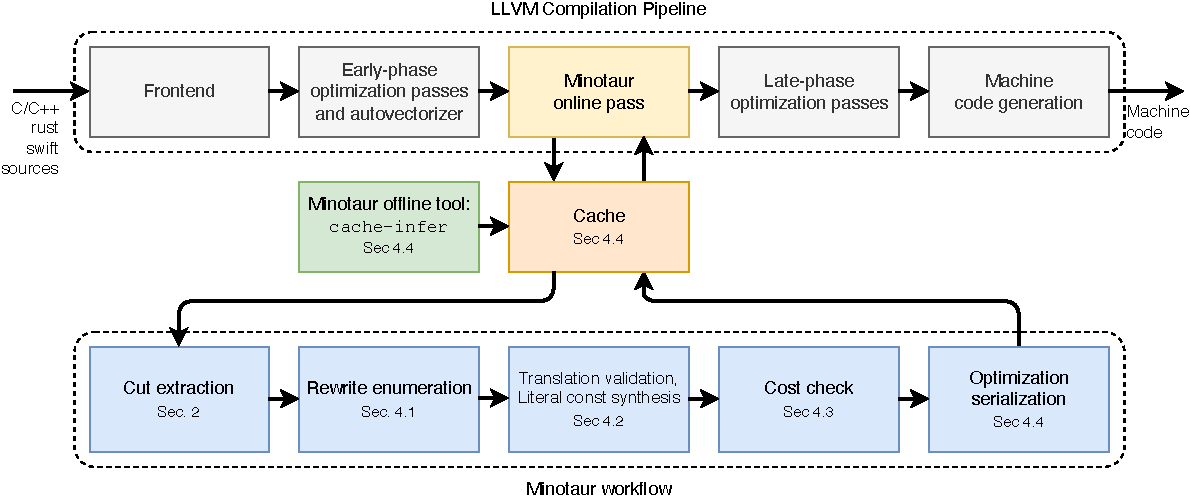
\includegraphics[width=\linewidth]{figures/flowchart.pdf}
    \caption{Overview of how \minotaur{} works.}
    \label{fig:workflow}
\end{figure}

Figure~\ref{fig:workflow} illustrates \minotaur's high-level structure,
and how it fits into LLVM\@.
%
It works by extracting many different \textit{cuts} from an LLVM function.
%
Each cut serves as the specification for a program synthesis
problem, where the objective is to synthesize a new cut that refines
the old one and is cheaper.
%
When such a cut is found, \minotaur{} uses it to rewrite the original
LLVM function, and also caches the rewrite.


Reasoning about the correctness of optimizations at the level of LLVM
IR can be very difficult; we have repurposed Alive2~\cite{alive2} to
serve as a verification backend.
%
To Alive2, we added formal semantics for Intel-architecture-specific
SIMD intrinsics.
%
Reasoning about the relative costs of code sequences is another
difficult problem; the solution adopted by \minotaur{} is to reuse the
LLVM Machine Code Analyzer~\cite{llvmmca}, which has adequately
accurate pipeline models for various modern processors.
%
These tools, along with the LLVM compiler itself, form the
foundation upon which \minotaur{} is built.


\textbf{Research contributions:}
%
First, we designed and implemented a domain-specific program
transformer that extracts an SSA value from an LLVM function, along
with context about how that value was computed.
%
Extracting enough context to permit interesting optimizations, without
extracting so much context that the underlying SMT solver was
overwhelmed, was an interesting empirical problem.
%
Second, we created a synthesis engine that searches for cheaper code
sequences; it enumerates partially symbolic candidates where the
instructions are concrete, but constants are symbolic.
%
For this part of our work, we created formal semantics for 165 LLVM
intrinsic functions that correspond to SIMD operations supported by
x86-64 processors, and added these to Alive2.
%
We also modified Alive2 to support synthesis of literal constants.
%
Third, to mitigate the large performance overhead of running program
synthesis at compile time, we developed infrastructure for caching
optimizations.
%
Thus, while \minotaur{} can be hundreds of times slower than \texttt{clang
  -O3} when its cache is cold, with a warm cache it is just 3\%
slower, when building the SPEC CPU 2017 benchmarks.



We performed a detailed evaluation of \minotaur's ability to speed up
code, showing that it can find numerous optimizations that LLVM fails
to perform, and also that it can achieve speedups on a variety of
real-world libraries and benchmarks.
%
\minotaur{} is also useful for compiler developers, and in fact several
optimizations it has discovered have now been implemented in upstream
LLVM\@.
